% PART IV — PHASE-WISE RESEARCH AND IMPLEMENTATION
\chapter{Chapter 6: 1M Breakthrough, Adaptive Control, and Multi-Task Scaling (Phases 12–15)}
\section{6.1 Phases 12–13.5: Dense 1M Convergence and OOD Slip Discovery}
Scaling dense potential shaping (Equation 10) to 1,000,000 steps in Phase 12 triggered an abrupt capability cascade between 300k and 500k steps: Reach (33\%->100\%), Grasp (20\%->100\%), Lift (1\%->98\%), and Placement (0\%->99\%), locking at 100\% through 1M steps with 0.0142 m final error and 89.84 hold steps (Figure 6.1). Extending training to DR1/DR2/DR4 in Phase 13 achieved 99–100\% Matched evaluation accuracy but revealed severe Held-Out DR4 collapse (57.0\% combined; Seed 43 only 33.0\%, Figure 6.2). Phase 13.5 forensics (1,520 episodes) captured the exact 68.4 N -> 0.0 N slip event under heavy mass (0.25 kg) and low friction (mu=0.3) (Figure 6.3).

\begin{figure}[htbp]\centering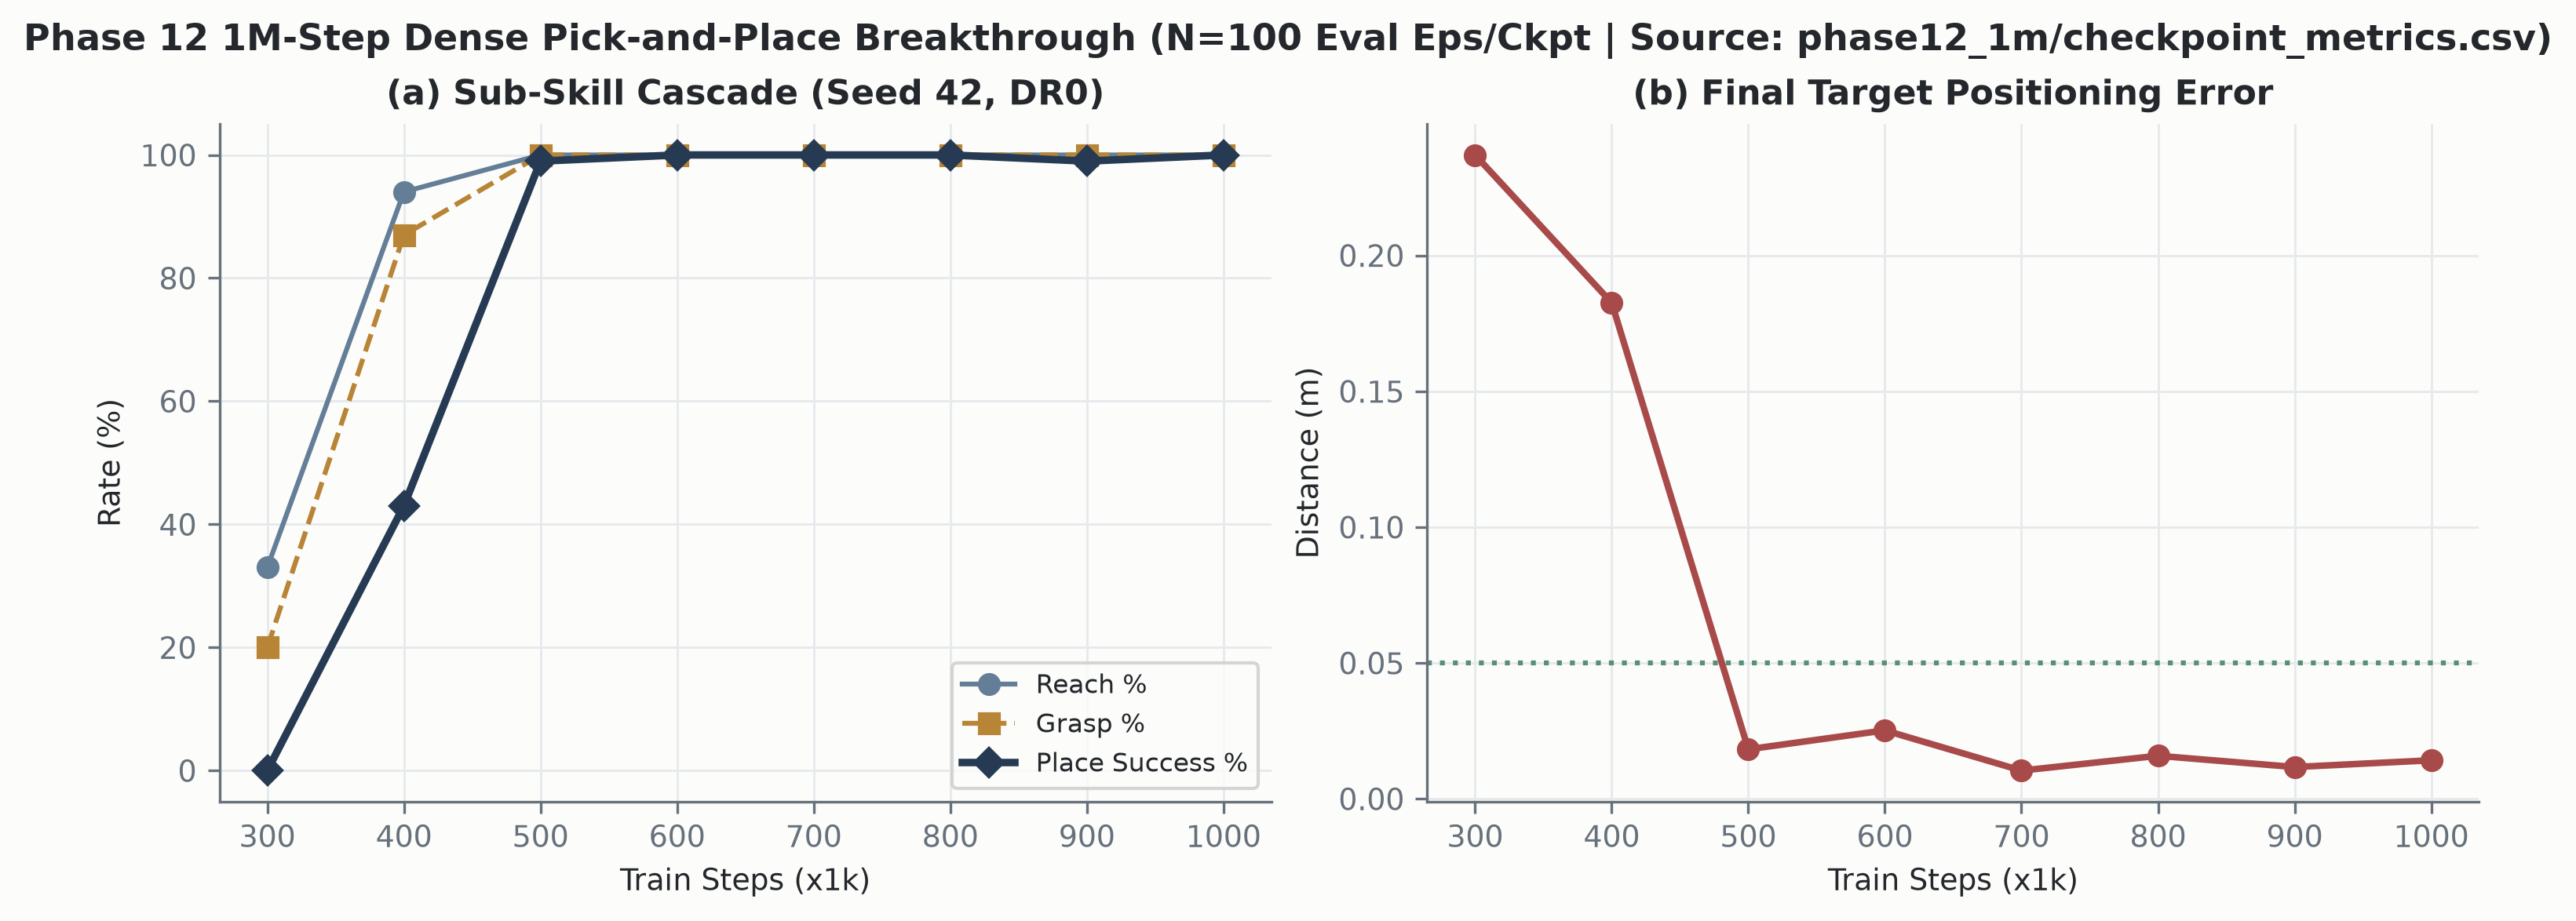
\includegraphics[width=0.9\linewidth]{../../assets/plots/plot_03_phase12_1m_breakthrough.png}\caption{Figure 6.1: Phase 12 1M-step dense Pick-and-Place S-curve (N=100 evaluation episodes per checkpoint, DR0 Seed 42).}\end{figure}
\begin{figure}[htbp]\centering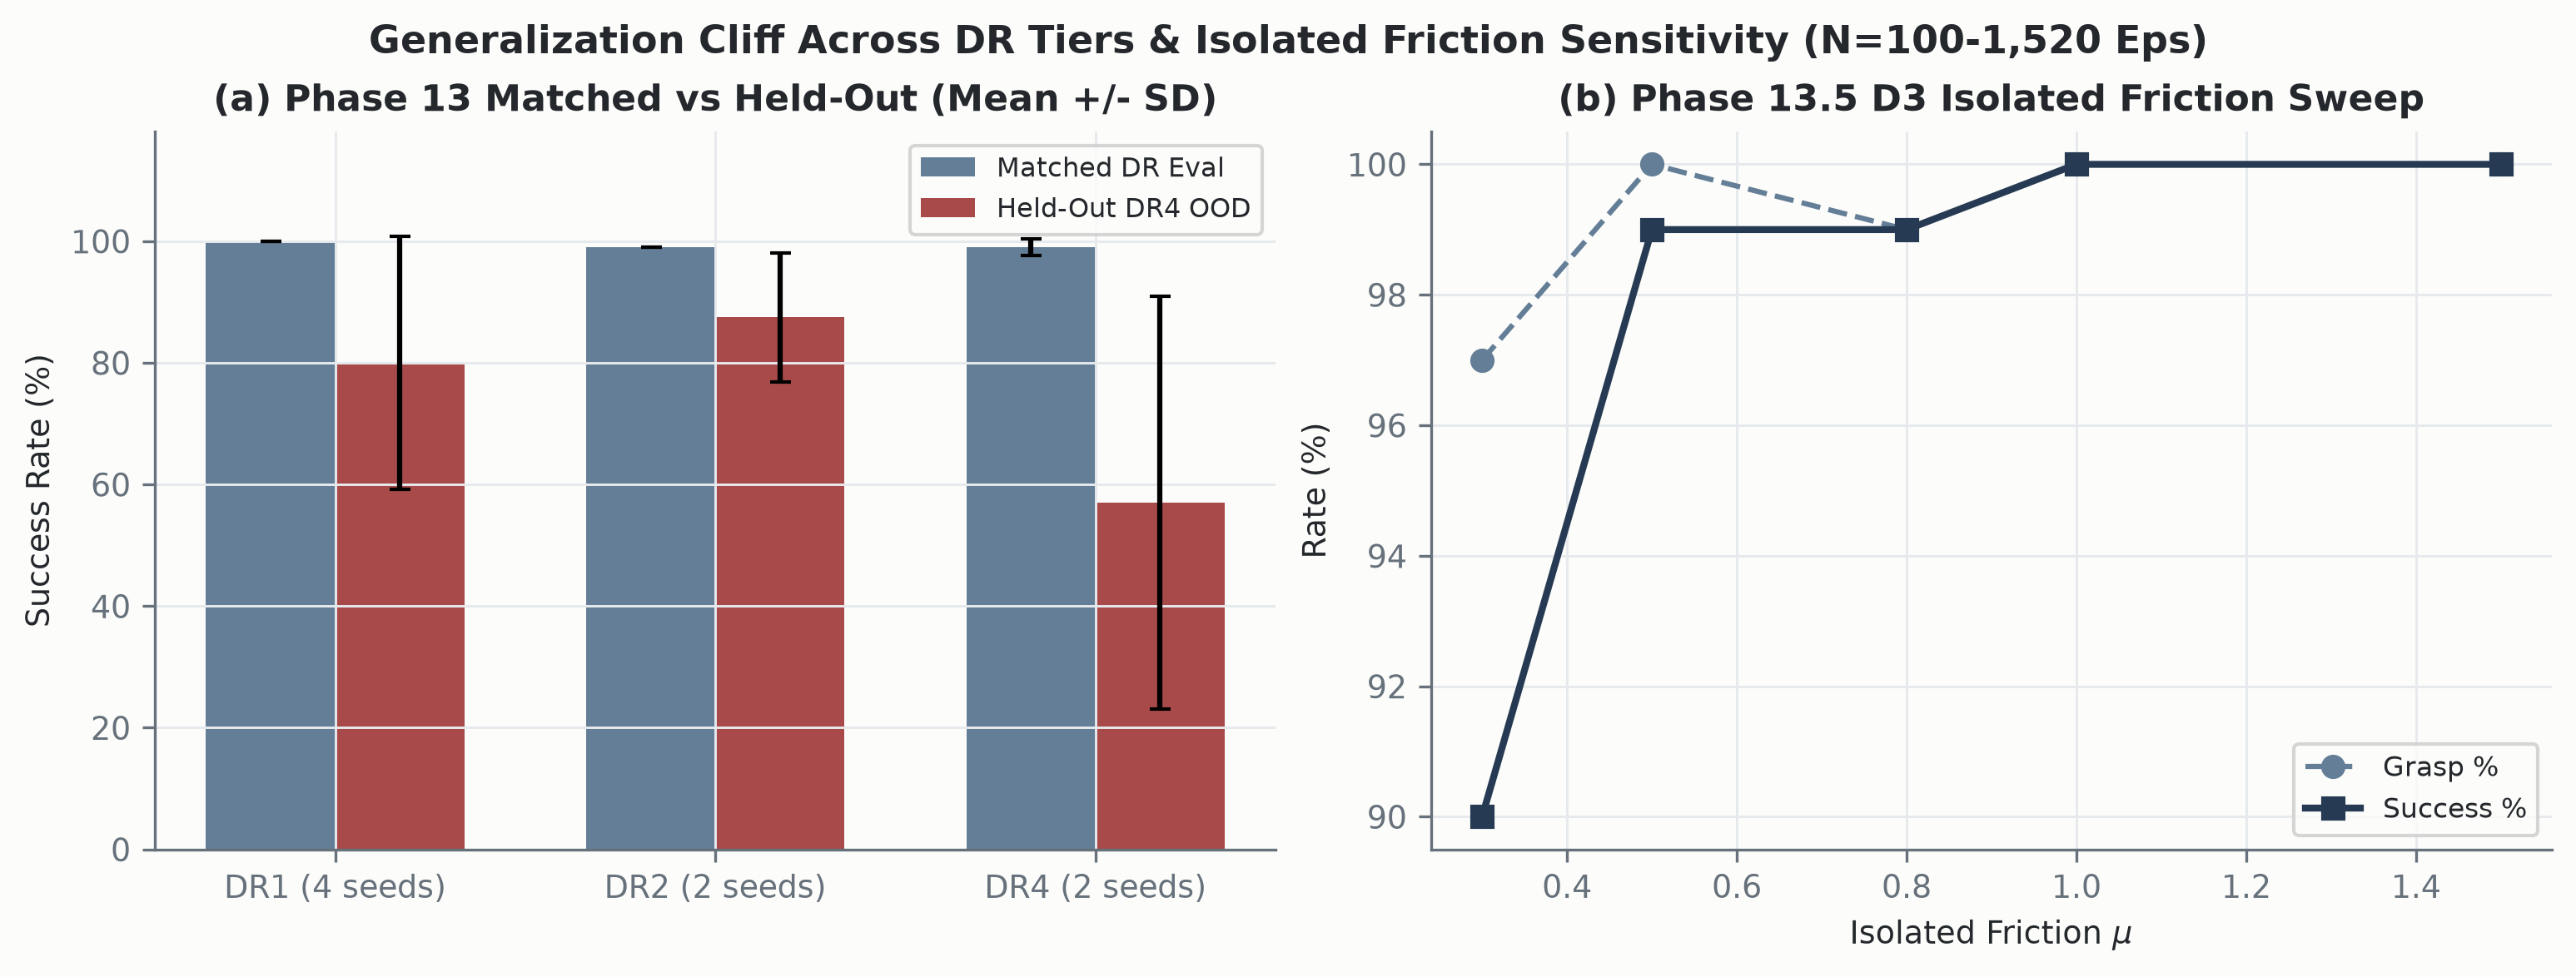
\includegraphics[width=0.9\linewidth]{../../assets/plots/plot_04_phase13_dr_with_errorbars.png}\caption{Figure 6.2: Phase 13 Matched vs. Held-Out DR4 generalization gap (multi-seed Mean +/- SD) and Phase 13.5 isolated friction sweep.}\end{figure}
\begin{figure}[htbp]\centering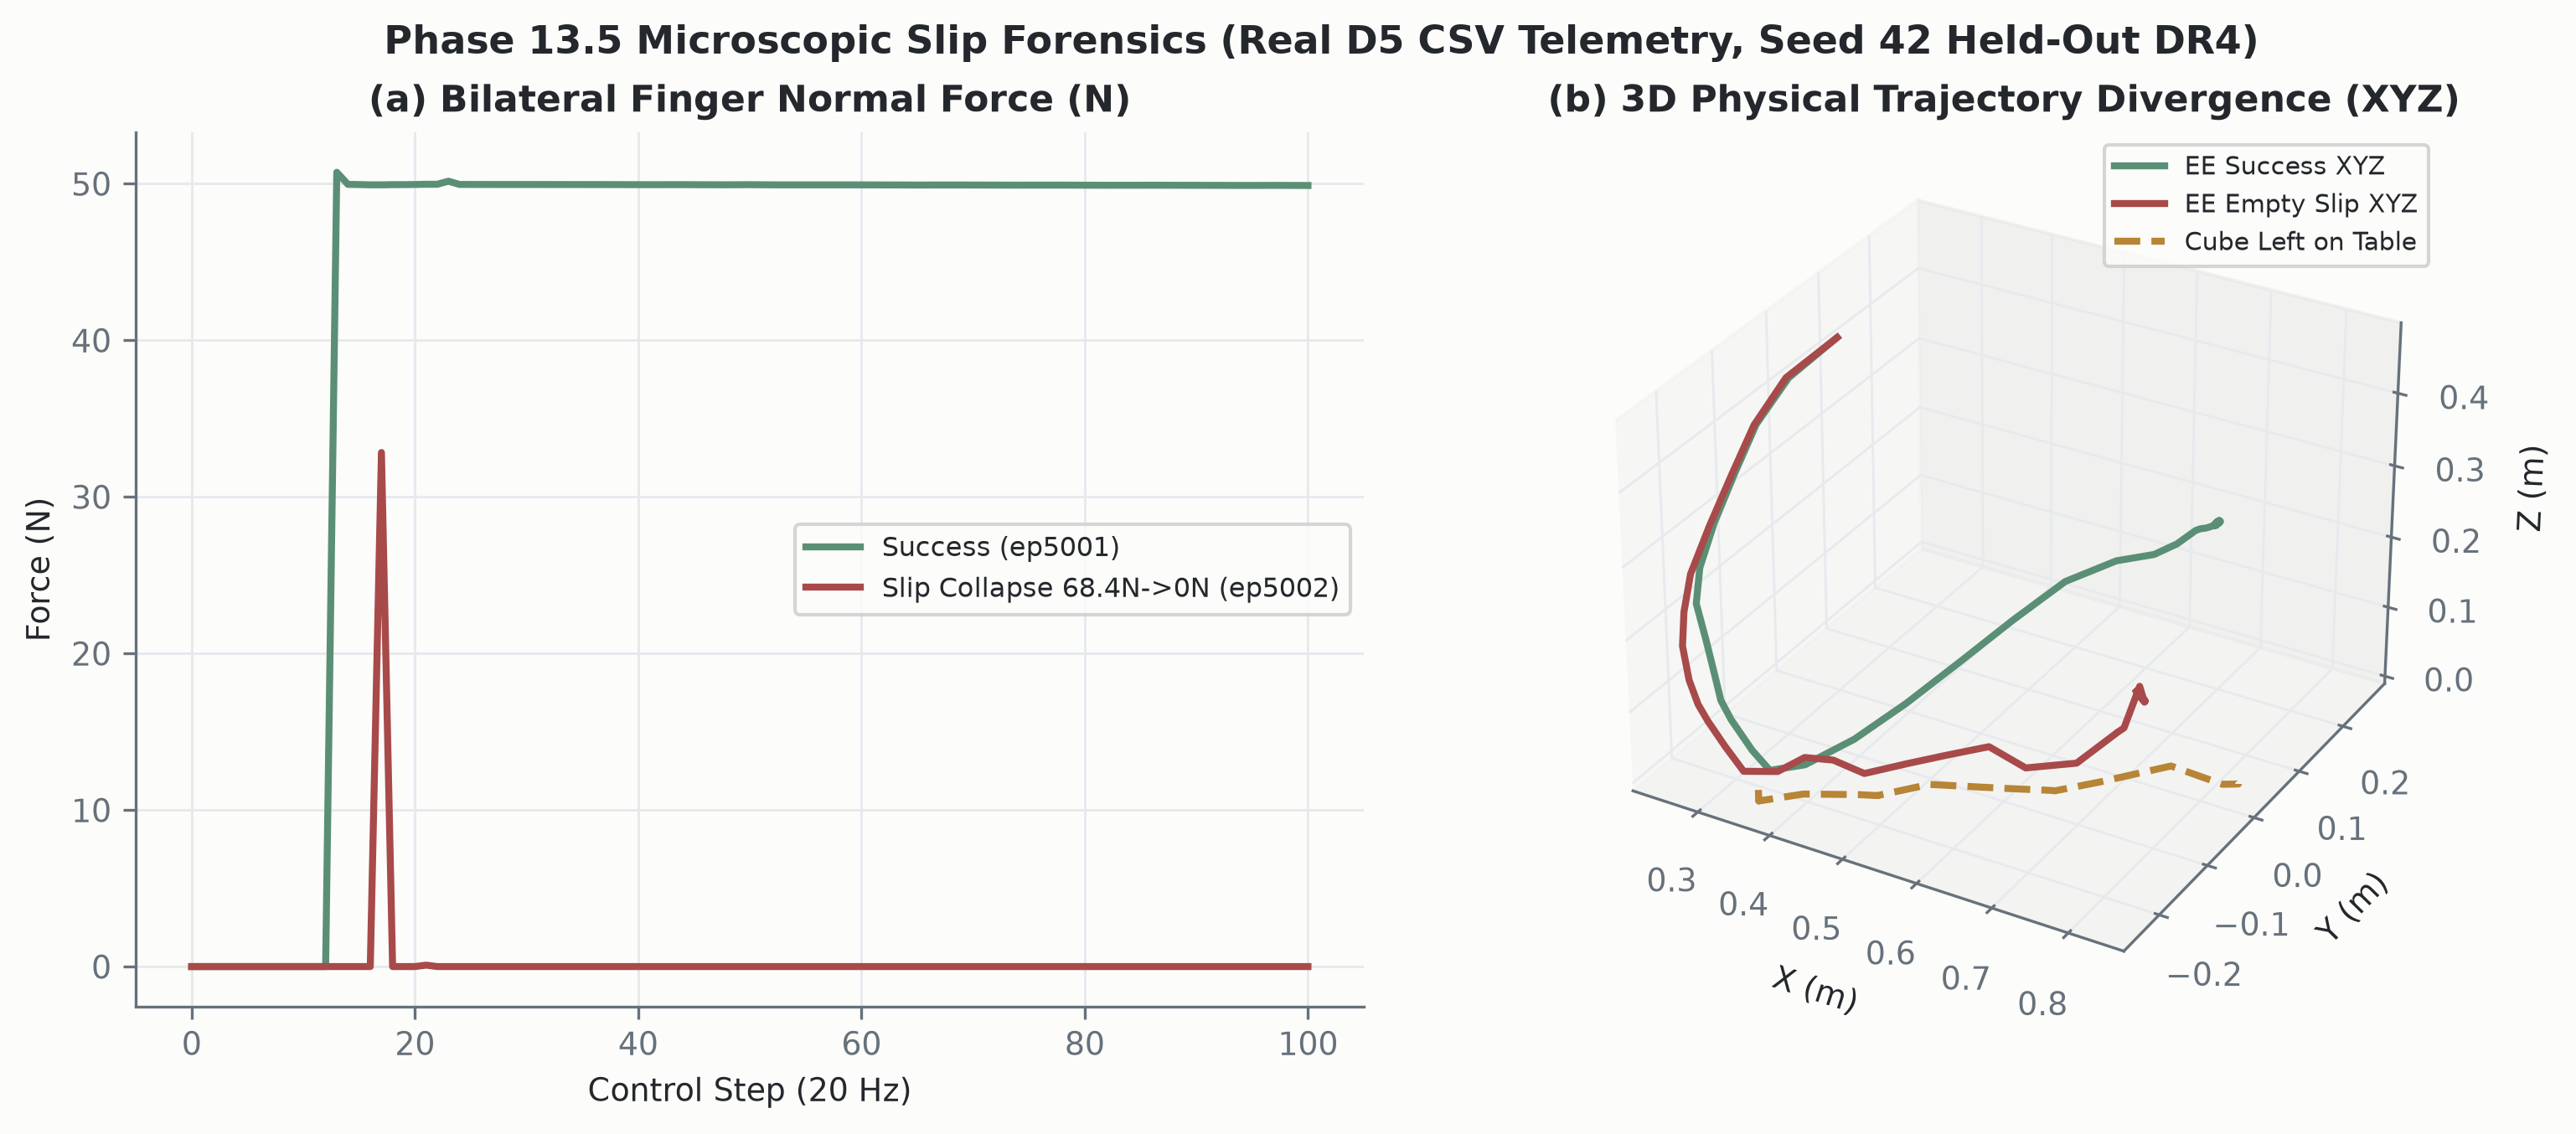
\includegraphics[width=0.9\linewidth]{../../assets/plots/plot_05_phase13_5_slip_telemetry_2d_3d.png}\caption{Figure 6.3: Real Phase 13.5 D5 telemetry contrasting successful lift (ep5001) against Stage-3 slip collapse (ep5002) in 2D \& 3D.}\end{figure}
\section{6.2 Phase 14: Zero-Retraining Adaptive Manipulation Shields (+41.0 pp Gain)}
To eliminate liftoff slip without retraining frozen neural weights, Phase 14 wrapped the policy output inside `AdaptiveTransportController` (Figure 6.4). Adding a 3-step zero-XY grasp settle floor (F\_n >= 5 N) and dynamic vertical velocity throttling propelled Held-Out DR4 confirmation (N=200 combined) from 57.0\% (Controller A) -> 89.5\% (Controller D) -> 98.0\% (Controller E), rescuing worst-case Seed 43 from 33.0\% to 99.0\% while retaining 100.0\% DR0 Nominal accuracy (Figure 6.5).

\begin{figure}[htbp]\centering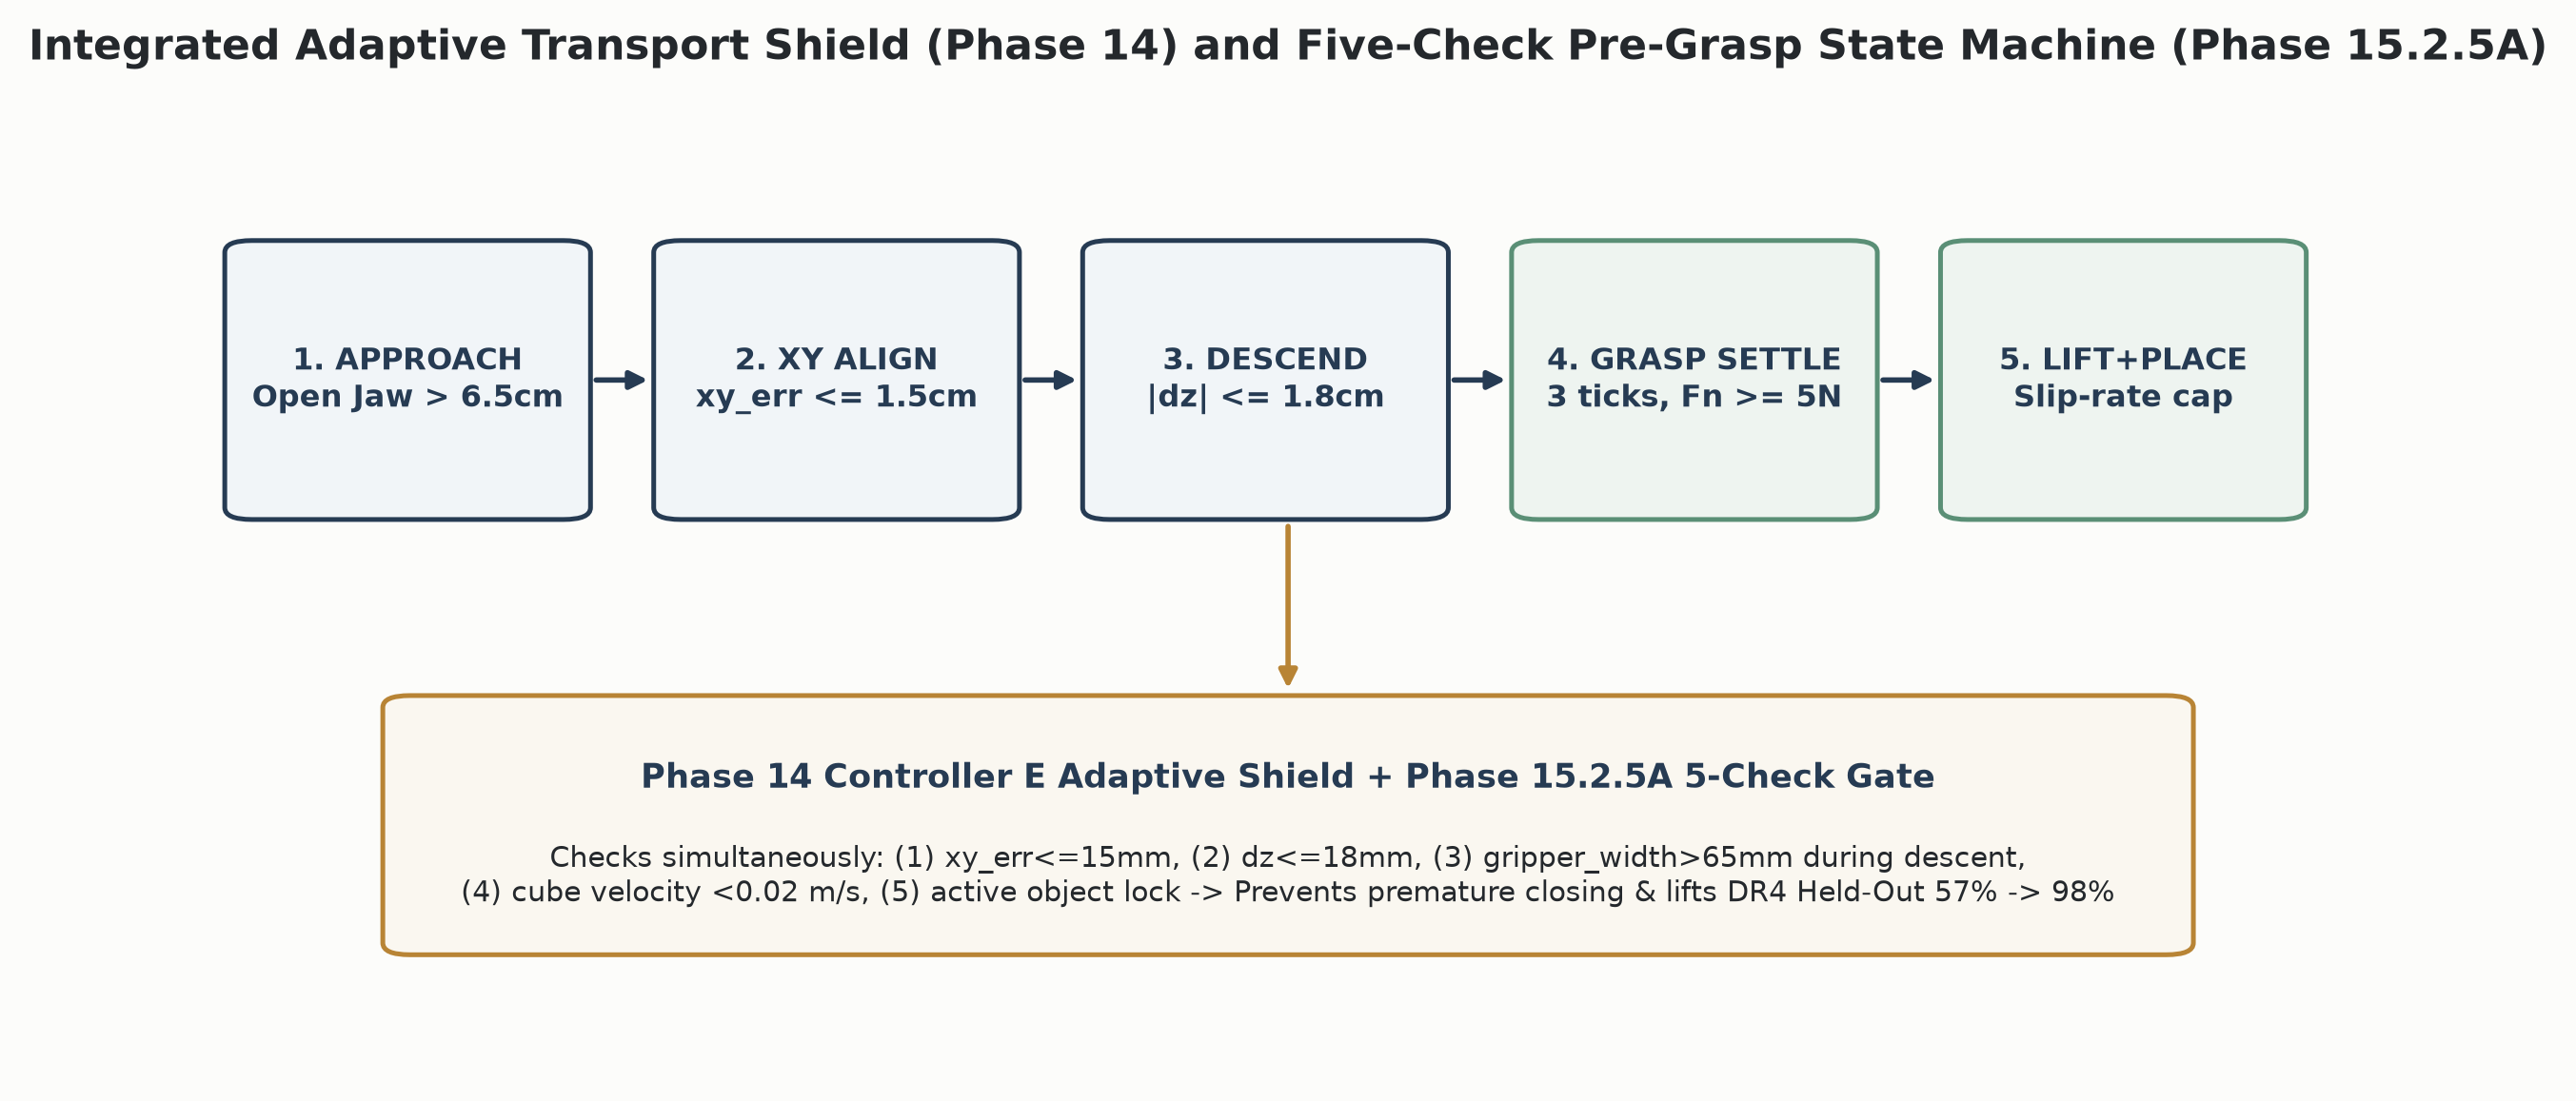
\includegraphics[width=0.9\linewidth]{../../assets/diagrams/diag_09_adaptive_shield_and_pregrasp.png}\caption{Figure 6.4: Phase 14 Adaptive Manipulation Shield integrated with the Phase 15.2.5A five-check bilateral PreGrasp FSM.}\end{figure}
\begin{figure}[htbp]\centering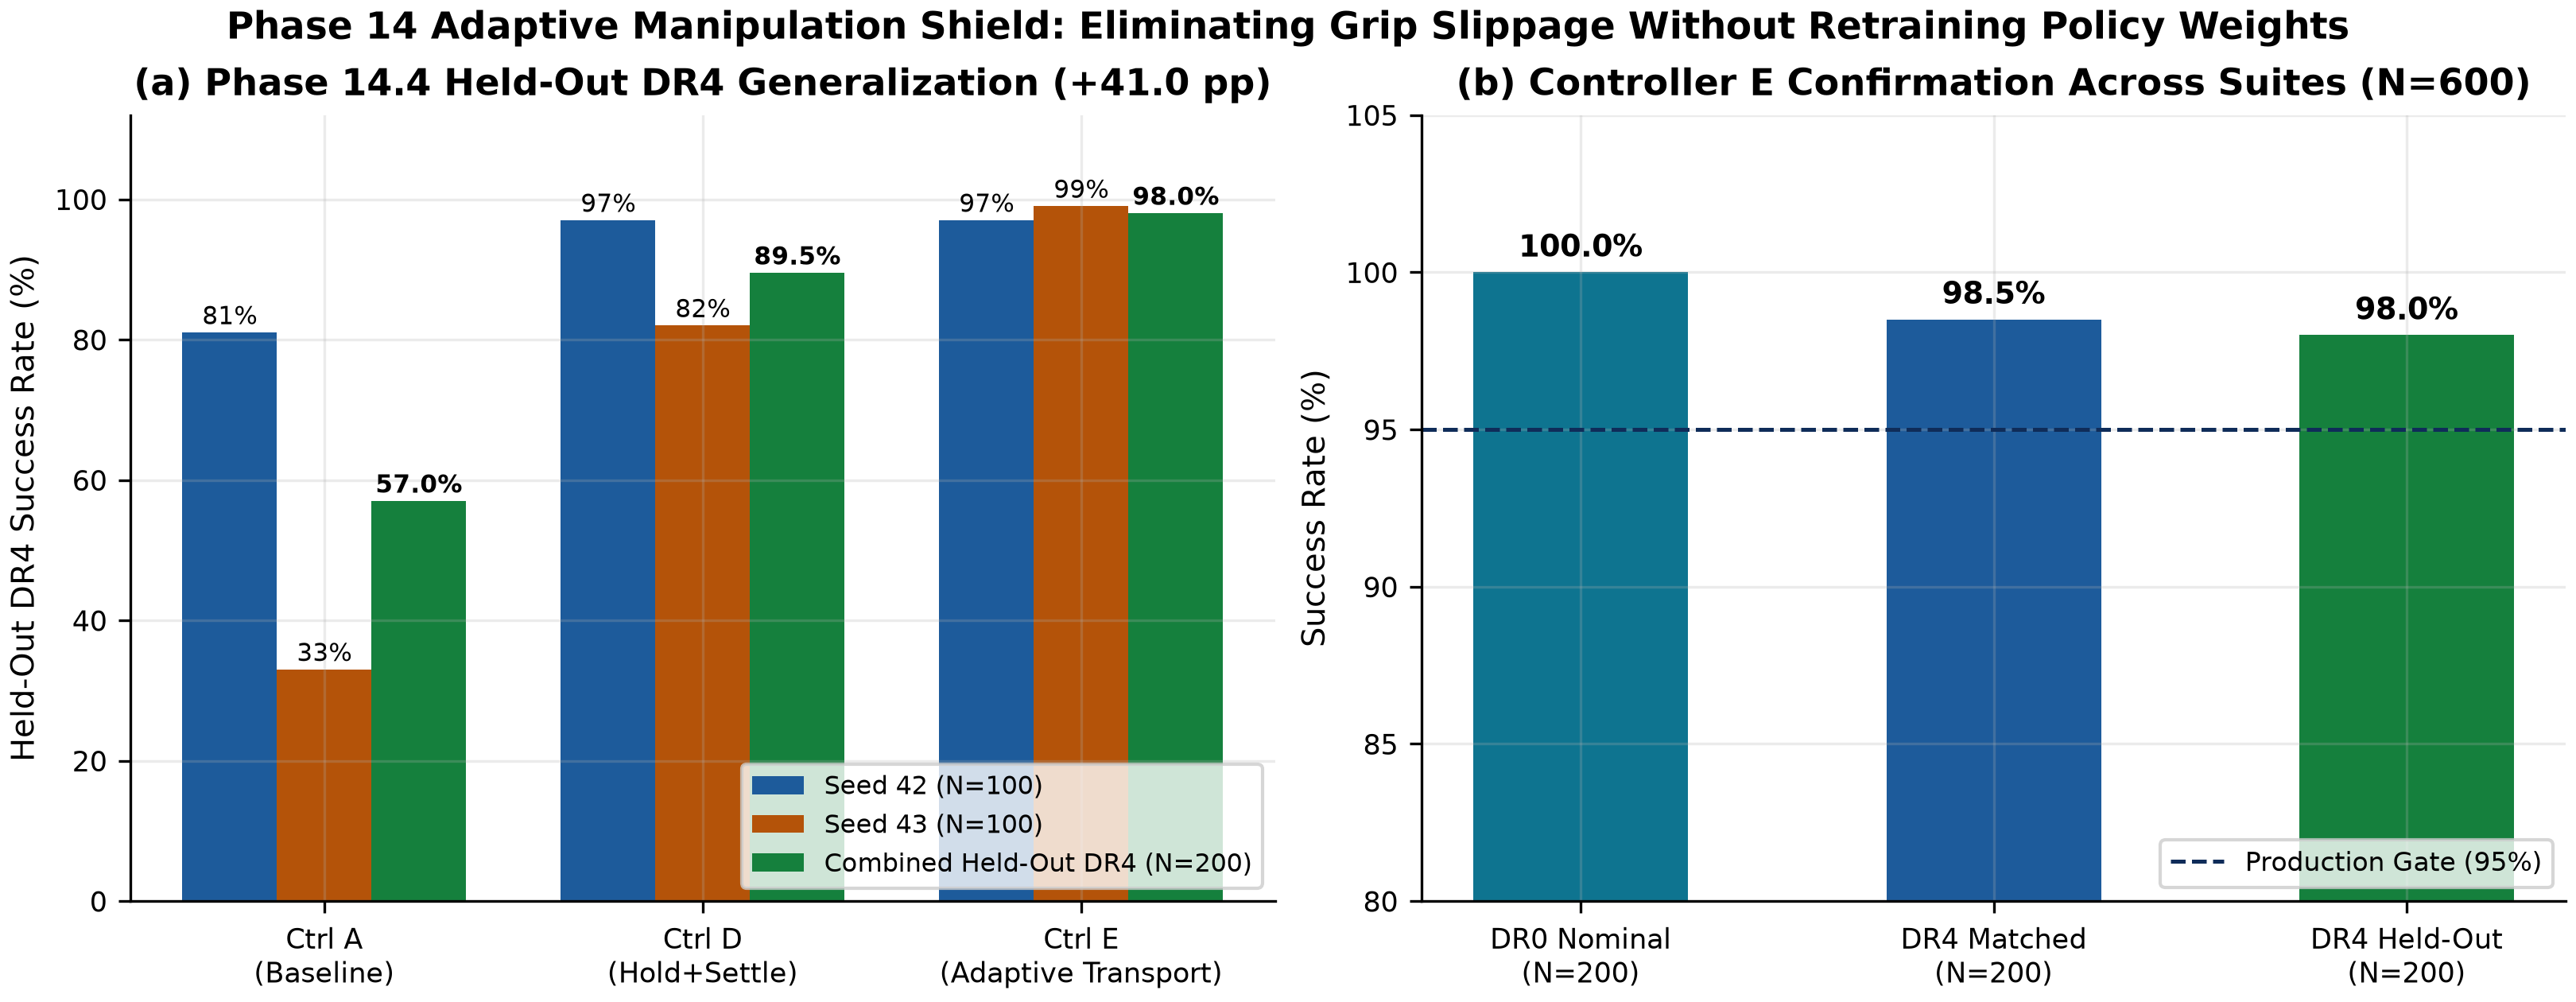
\includegraphics[width=0.9\linewidth]{../../assets/plots/plot_06_phase14_controllers_comparison.png}\caption{Figure 6.5: Phase 14.4 Held-Out DR4 confirmation across Controllers A, D, and E (Seeds 42, 43, and N=200/600 combined suites).}\end{figure}
\section{6.3 Phase 15: Perturbation Sensitivity, Pre-Grasp Sorting \& Masked BC-SAC}
Phase 15.1 evaluated Controller E across 320 perturbed episodes: ±3 mm (97.5\%) and ±5 mm (95.0\%) spatial noise remained robust, 1-step delay dropped to 72.5\%, >=2-step delay collapsed to 0.0\%, and stripping oracle forces fell to 42.5\%. Phase 15.2.5A achieved 50/50 (100\%) scripted two-object sorting (76.4 steps, 0 collisions, Figure 6.6a), whereas single-object RL ablations 5B2–5B8 proved pure masked BC (5B7: 75\% grasp / 45\% lift, 0\% coll) outperformed pure 17.5k SAC (5B2: 62\%/7\%) and Hybrid BC-SAC (5B8: 66\%/26\%) on 100 unseen episodes. Multi-object RL transfer (Phase 15.2.5C) remained BLOCKED; Phase 15.3 scripted assembly scored 56.67\% vs 23.33\% BC pre-align (Figure 6.7).

\begin{figure}[htbp]\centering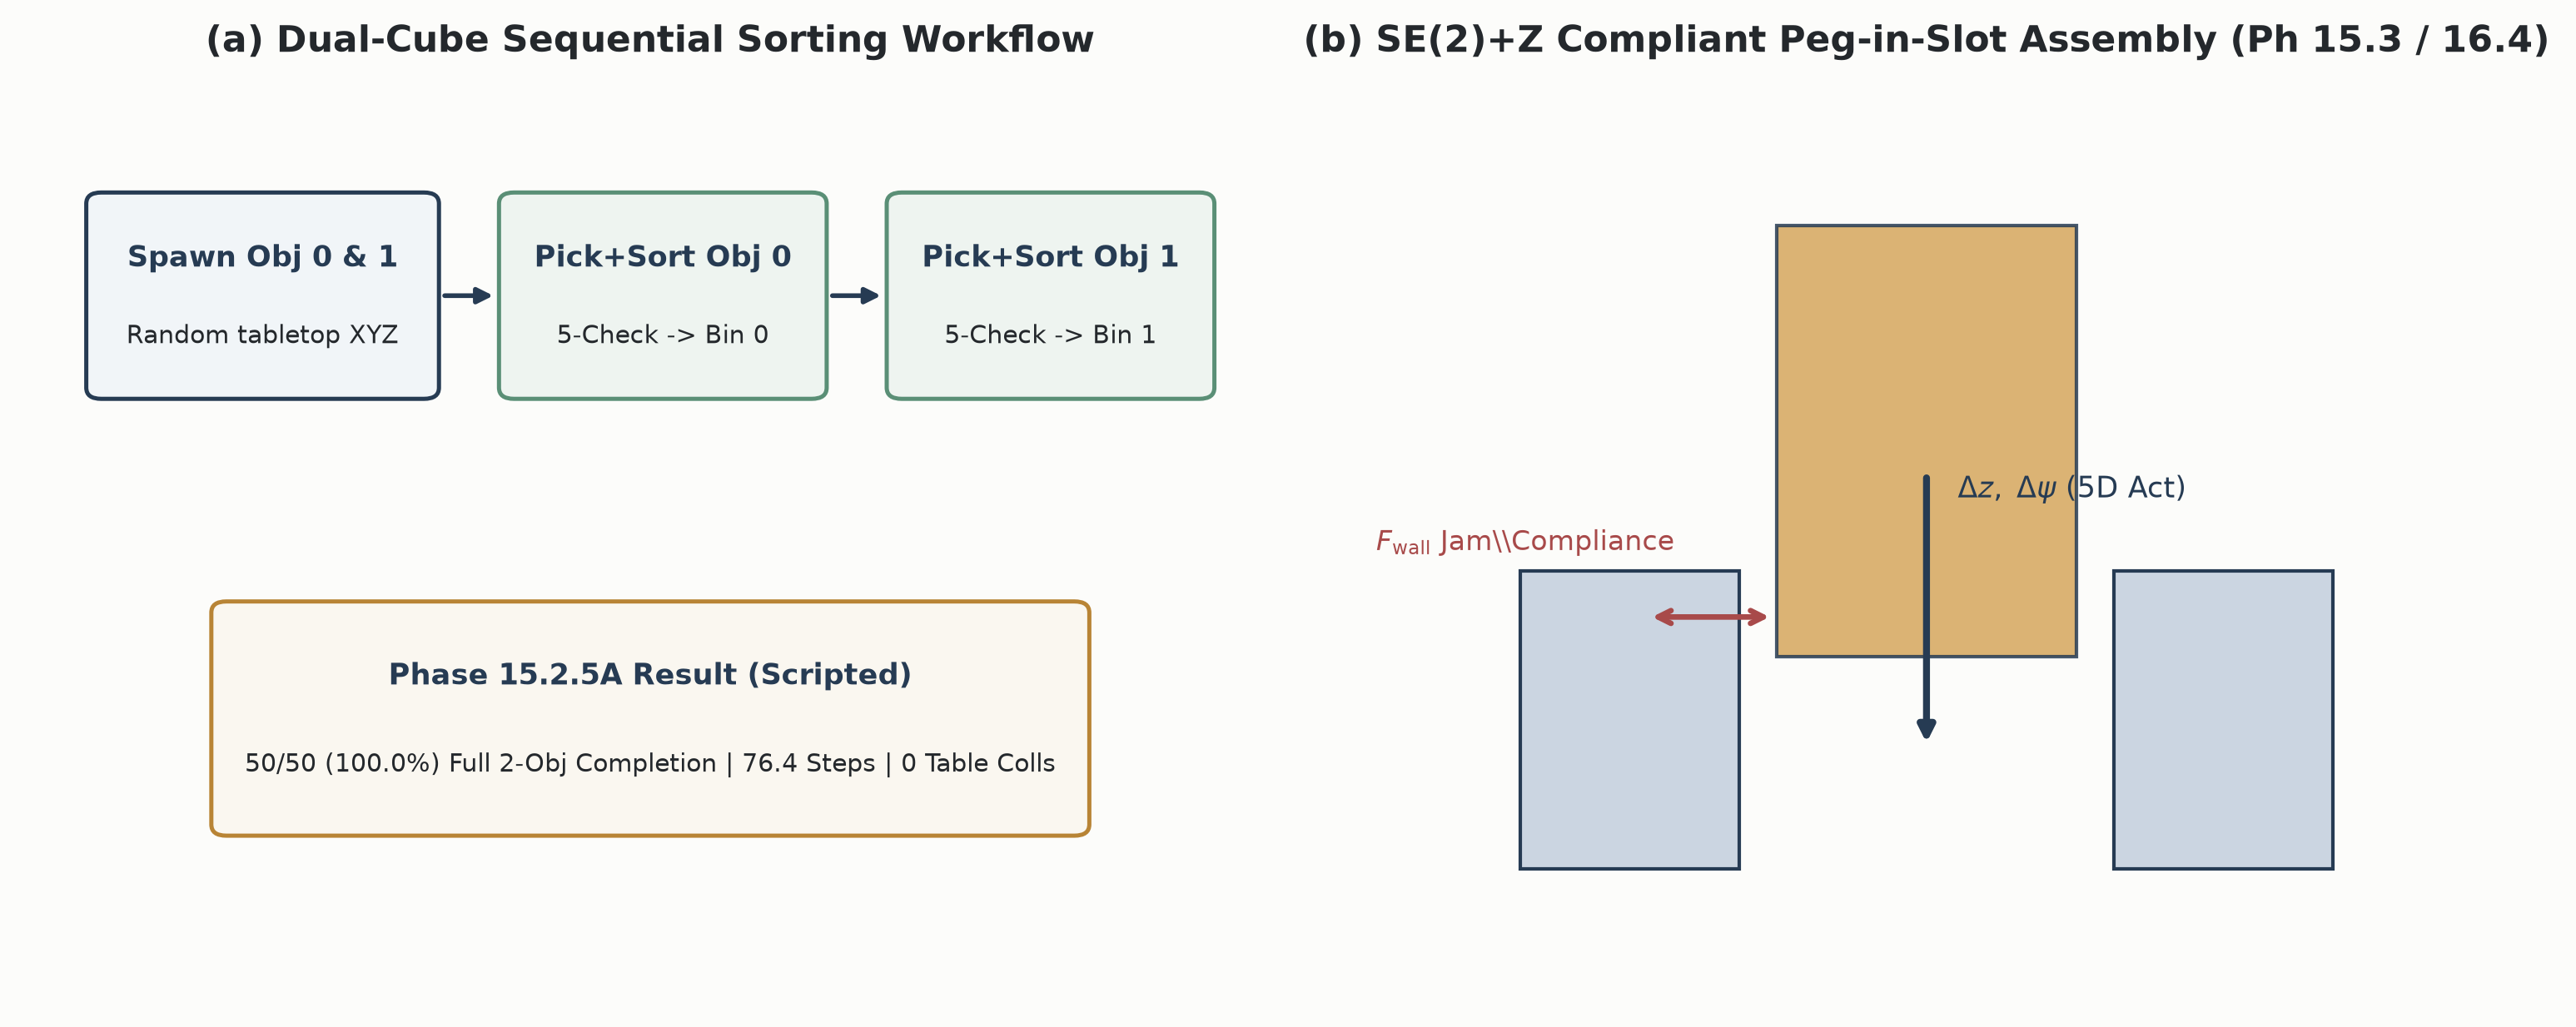
\includegraphics[width=0.9\linewidth]{../../assets/diagrams/diag_10_task_lifecycles_multisort_assembly.png}\caption{Figure 6.6: Sequential dual-cube MultiSort workflow (50/50 scripted) and SE(2)+Z compliant peg-in-slot insertion geometry.}\end{figure}
\begin{figure}[htbp]\centering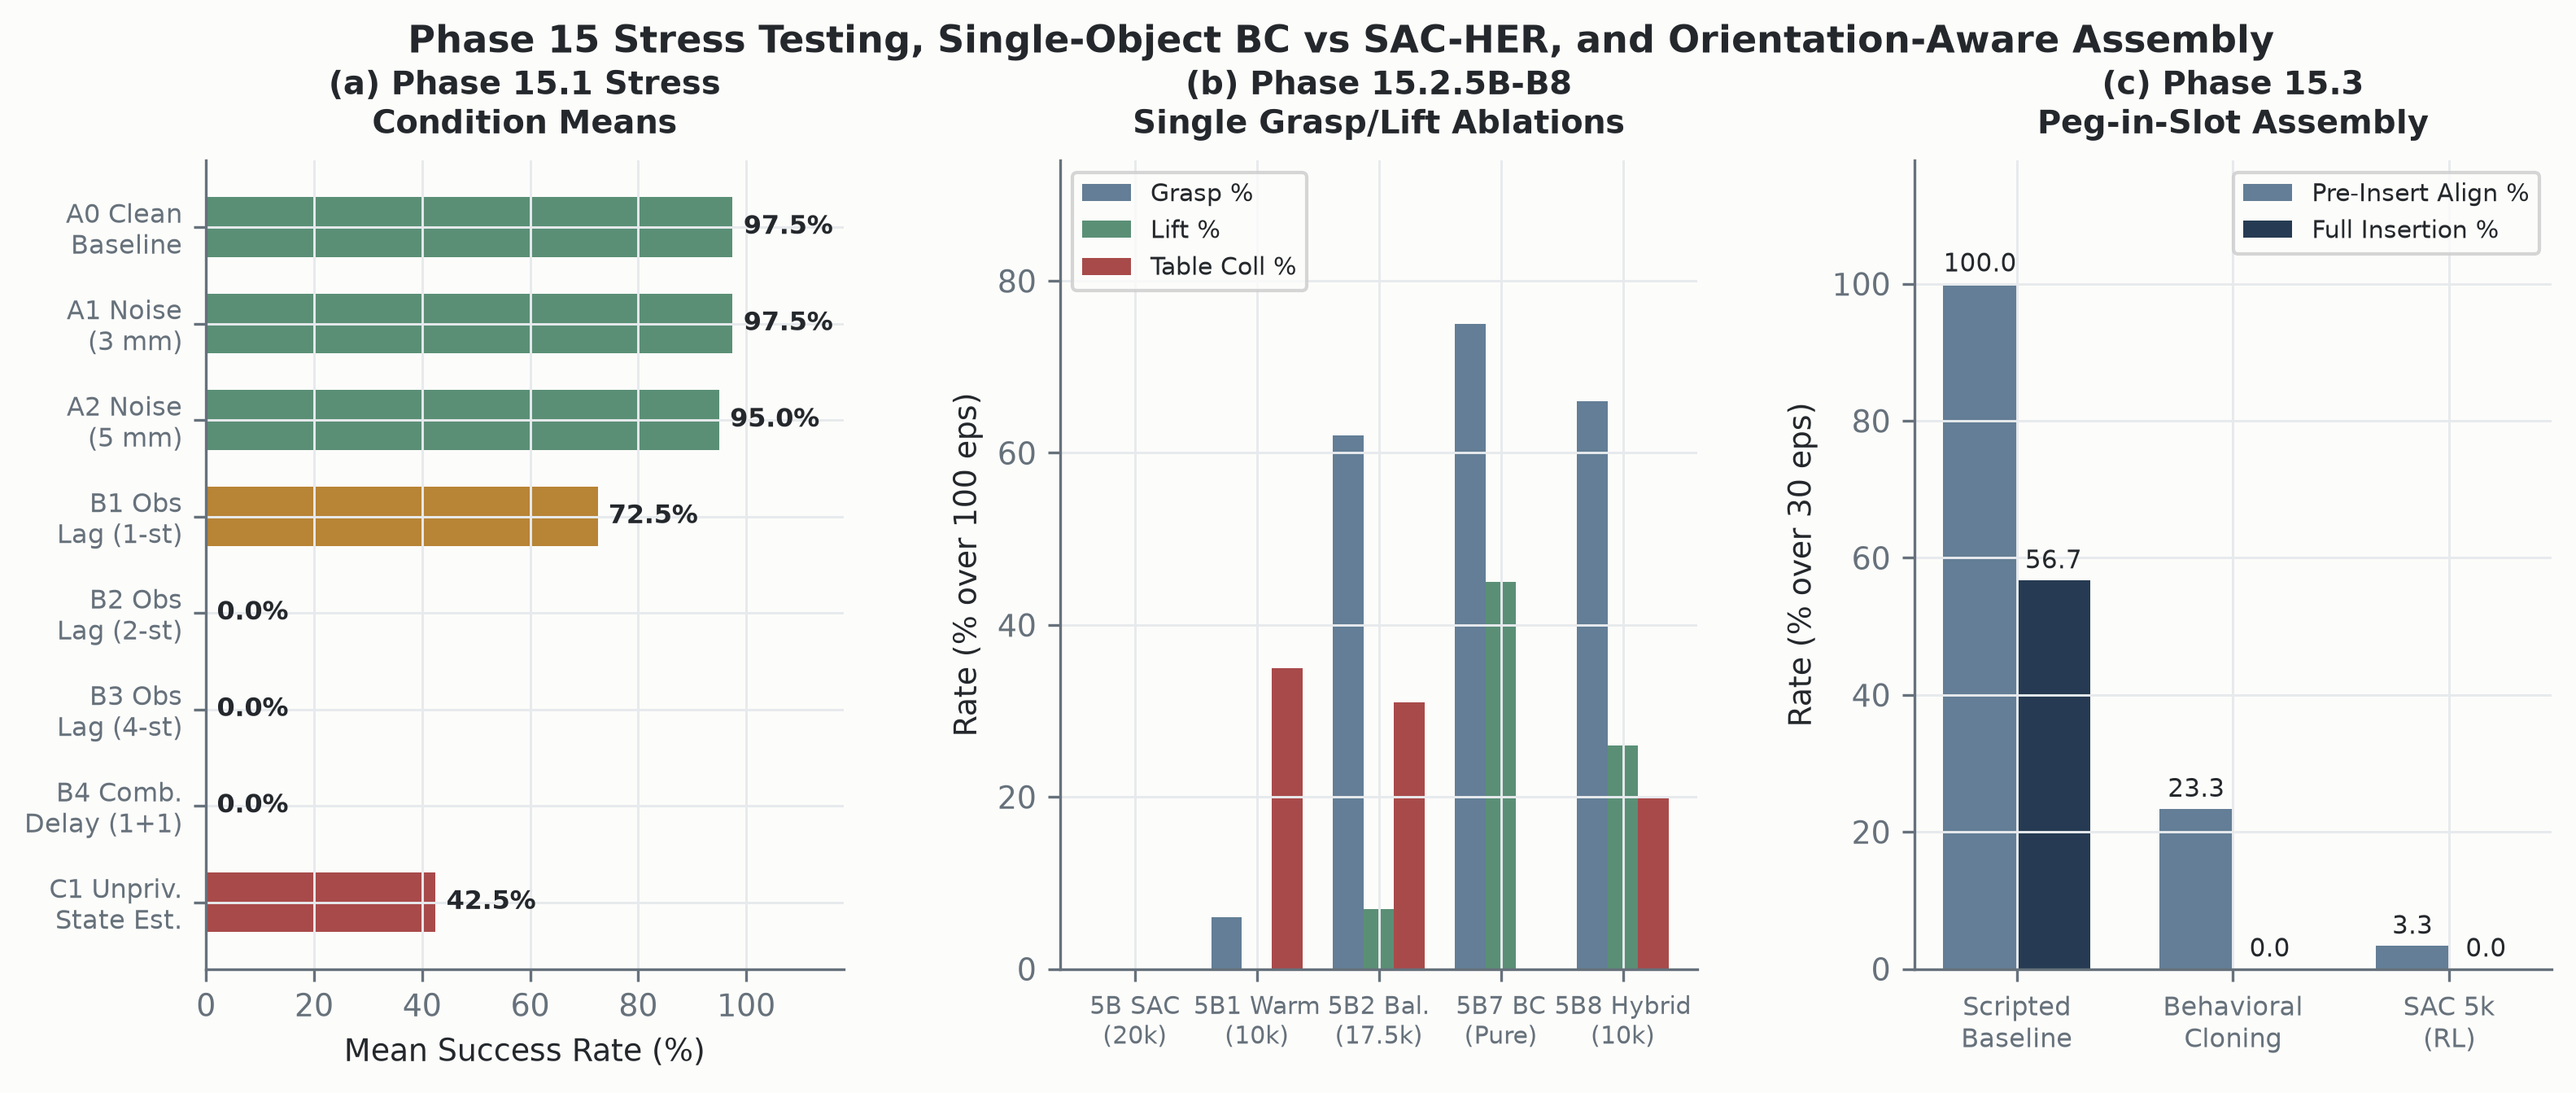
\includegraphics[width=0.9\linewidth]{../../assets/plots/plot_07_phase15_ablations_and_stress.png}\caption{Figure 6.7: Phase 15.1 stress resilience, 15.2.5B–B8 grasp/lift ablations, and Phase 15.3 assembly results.}\end{figure}